\documentclass{beamer}
\usepackage[utf8]{inputenc}
\usepackage[english]{babel}
\usepackage[T1]{fontenc}
\usepackage[inline]{asymptote}
\usepackage{pgfplots}
\pgfplotsset{compat=1.5} 
\usepgfplotslibrary{statistics}
\usepackage{graphicx}
\usepackage{subcaption}
\usepackage{slide_helper}

\pgfplotsset{ every non boxed x axis/.append style={x axis line style=-},
     every non boxed y axis/.append style={y axis line style=-}}

\title[MA205 - Section 2.3]{Graphs That Enlighten and Graphs That Deceive}

\newcommand{\textsep}{\vspace{0.5mm}}

\begin{document}
\begin{frame}
\titlepage
\end{frame}

\begin{frame}
\begin{definition}
A \textbf{dotplot} consists of a graph of quantitative data in which each data value is plotted as a point above a horizontal scale of values. Dots representing equal values are stacked.
\end{definition}\pause

\begin{block}{Features}
\begin{itemize}
\item Displays the shape of the distribution of data.
\item It is usually possible to recreate the original list of data values.
\end{itemize}
\end{block}
\end{frame}

\begin{frame}
\begin{example}
The dotplot shows the pulse rates (beats per minute) of males.\\(Data Set 1 in Appendix B.)
\begin{center}
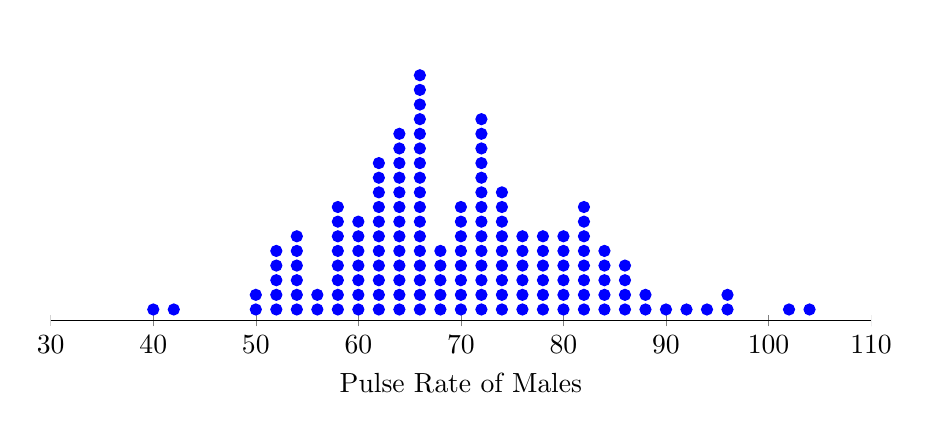
\begin{tikzpicture}
\begin{axis}[
width=12cm,
height=5.3cm,
xlabel={Pulse Rate of Males},
ylabel={},
yticklabels={},
axis y line=none,
axis x line=bottom,
ymin=0,
ymax=20,
xmin=30,
xmax=110,
scatter/use mapped color={
 %draw=mapped color,
 fill=blue,
},
]
\addplot[scatter, only marks, blue, scatter src=y]
coordinates
{
(40, 0.75)
(42, 0.75)
(50, 0.75)
(50, 1.75)
(52, 0.75)
(52, 1.75)
(52, 2.75)
(52, 3.75)
(52, 4.75)
(54, 0.75)
(54, 1.75)
(54, 2.75)
(54, 3.75)
(54, 4.75)
(54, 5.75)
(56, 0.75)
(56, 1.75)
(58, 0.75)
(58, 1.75)
(58, 2.75)
(58, 3.75)
(58, 4.75)
(58, 5.75)
(58, 6.75)
(58, 7.75)
(60, 0.75)
(60, 1.75)
(60, 2.75)
(60, 3.75)
(60, 4.75)
(60, 5.75)
(60, 6.75)
(62, 0.75)
(62, 1.75)
(62, 2.75)
(62, 3.75)
(62, 4.75)
(62, 5.75)
(62, 6.75)
(62, 7.75)
(62, 8.75)
(62, 9.75)
(62, 10.75)
(64, 0.75)
(64, 1.75)
(64, 2.75)
(64, 3.75)
(64, 4.75)
(64, 5.75)
(64, 6.75)
(64, 7.75)
(64, 8.75)
(64, 9.75)
(64, 10.75)
(64, 11.75)
(64, 12.75)
(66, 0.75)
(66, 1.75)
(66, 2.75)
(66, 3.75)
(66, 4.75)
(66, 5.75)
(66, 6.75)
(66, 7.75)
(66, 8.75)
(66, 9.75)
(66, 10.75)
(66, 11.75)
(66, 12.75)
(66, 13.75)
(66, 14.75)
(66, 15.75)
(66, 16.75)
(68, 0.75)
(68, 1.75)
(68, 2.75)
(68, 3.75)
(68, 4.75)
(70, 0.75)
(70, 1.75)
(70, 2.75)
(70, 3.75)
(70, 4.75)
(70, 5.75)
(70, 6.75)
(70, 7.75)
(72, 0.75)
(72, 1.75)
(72, 2.75)
(72, 3.75)
(72, 4.75)
(72, 5.75)
(72, 6.75)
(72, 7.75)
(72, 8.75)
(72, 9.75)
(72, 10.75)
(72, 11.75)
(72, 12.75)
(72, 13.75)
(74, 0.75)
(74, 1.75)
(74, 2.75)
(74, 3.75)
(74, 4.75)
(74, 5.75)
(74, 6.75)
(74, 7.75)
(74, 8.75)
(76, 0.75)
(76, 1.75)
(76, 2.75)
(76, 3.75)
(76, 4.75)
(76, 5.75)
(78, 0.75)
(78, 1.75)
(78, 2.75)
(78, 3.75)
(78, 4.75)
(78, 5.75)
(80, 0.75)
(80, 1.75)
(80, 2.75)
(80, 3.75)
(80, 4.75)
(80, 5.75)
(82, 0.75)
(82, 1.75)
(82, 2.75)
(82, 3.75)
(82, 4.75)
(82, 5.75)
(82, 6.75)
(82, 7.75)
(84, 0.75)
(84, 1.75)
(84, 2.75)
(84, 3.75)
(84, 4.75)
(86, 0.75)
(86, 1.75)
(86, 2.75)
(86, 3.75)
(88, 0.75)
(88, 1.75)
(90, 0.75)
(92, 0.75)
(94, 0.75)
(96, 0.75)
(96, 1.75)
(102, 0.75)
(104, 0.75)
};
\end{axis}
\end{tikzpicture}
\end{center}
\end{example}\pause

\begin{block}{Note}
A Histogram counts how many data values fall within an interval.\\ A Dotplot counts individual data points.
\end{block}
\end{frame}

\begin{frame}
\begin{definition}
A \textbf{stemplot} ( or \textbf{stem-and-leaf plot}) represents quantitative data by separating each value into two parts: % chktex 37
\begin{description}
\item[\textbf{The Stem:}] Usually the leftmost digit.
\item[\textbf{The Leaf:}] Usually the rightmost digits.
\end{description}
\end{definition}\pause

\begin{block}{Note}
You may have to round data values first.
\end{block}\pause

\begin{block}{Features}
\begin{itemize}
\item Shows the shape and distribution of the data.
\item Retains the original data values.
\item The sample data are sorted.
\end{itemize}
\end{block}
\end{frame}

\begin{frame}
\begin{example}
The stemplot shows the pulse rates (beats per minute) of males.\\(Data Set 1 in Appendix B.)
\begin{center}
\begin{tabular}{l|l}
4 & 02 \\
5 & 00222224444446688888888 \\
6 & 0000000222222222224444444444444666666666666666688888 \\
7 & 0000000022222222222222444444444666666888888 \\
8 & 0000002222222244444666688 \\
9 & 02466 \\
10 & 24
\end{tabular}
\end{center}
The left is the rightmost digits, the stem is all the remaining leftmost digits. The stems are listed in increasing order, not the order in which they occur in the dataset.
\end{example}
\end{frame}

\begin{frame}
\begin{definition}
A \textbf{time series graph} is a graph of quantitative data that have been collected at different points in time.
\end{definition}\pause

\begin{block}{Features}
\begin{itemize}
\item Reveals information about trends over time.
\end{itemize}
\end{block}
\end{frame}

\begin{frame}
\begin{example}
The time-series graph depicts the yearly number of fatalities of law enforcement officers in the United States.
\begin{center}
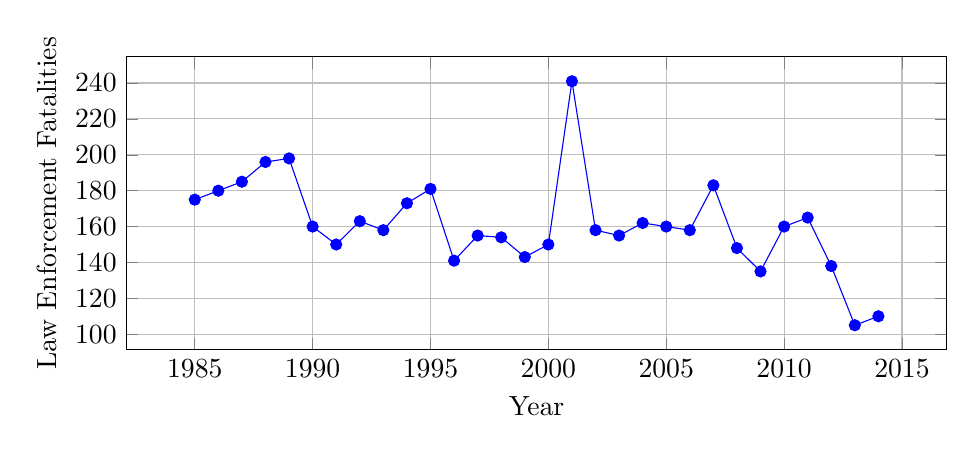
\begin{tikzpicture}
\pgfkeys{/pgf/number format/.cd,
fixed,
precision=999,
set thousands separator={},
1000 sep in fractionals=false,
}
\begin{axis}[
width=12cm,
height=5.3cm,
xlabel={Year},
ylabel={Law Enforcement Fatalities},
ymajorgrids=true,
xmajorgrids=true,
xticklabel style={/pgf/number format/.cd,fixed,precision=0},
xticklabel=\pgfmathprintnumber{\tick},
ytick={100,120,...,280},
%ymin=0,
%ymax=20,
%xmin=30,
%xmax=110,
scatter/use mapped color={
 %draw=mapped color,
 fill=blue,
},
]
\addplot[scatter, blue, scatter src=y]
coordinates
{
(1985, 175)
(1986, 180)
(1987, 185)
(1988, 196)
(1989, 198)
(1990, 160)
(1991, 150)
(1992, 163)
(1993, 158)
(1994, 173)
(1995, 181)
(1996, 141)
(1997, 155)
(1998, 154)
(1999, 143)
(2000, 150)
(2001, 241)
(2002, 158)
(2003, 155)
(2004, 162)
(2005, 160)
(2006, 158)
(2007, 183)
(2008, 148)
(2009, 135)
(2010, 160)
(2011, 165)
(2012, 138)
(2013, 105)
(2014, 110)
};
\end{axis}
\end{tikzpicture}
\end{center}\pause

Notice that there is a large spike in 2001, most of these fatalities would have been during the terrorist attacks on September 11, 2001. If we exclude the spike, there appears to be a slight downward trend.
\end{example}
\end{frame}

\begin{frame}
\begin{definition}
A \textbf{bar graph} uses bars of equal width to show frequencies of categories or categorical data. The bars may or may not be separated by small gaps.
\end{definition}\pause

\begin{block}{Features}
\begin{itemize}
\item Shows the relative distribution of categorical data so that it is easier to compare the different categories.
\end{itemize}
\end{block}\pause

\begin{definition}
A \textbf{Pareto chart} is a bar graph for categorical data, with the added stipulation that the bars are arranged in descending order according to the frequencies, so the bars decrease in height from left to right.
\end{definition}\pause

\begin{block}{Features}
\begin{itemize}
\item Shows the relative distribution of categorical data so that it is easier to compare the different categories.
\item Draws attention to the more important categories.
\end{itemize}
\end{block}
\end{frame}

\begin{frame}
\begin{example}
For the boats stolen in a recent year, the bar graph shows the types most often stolen.

\begin{center}

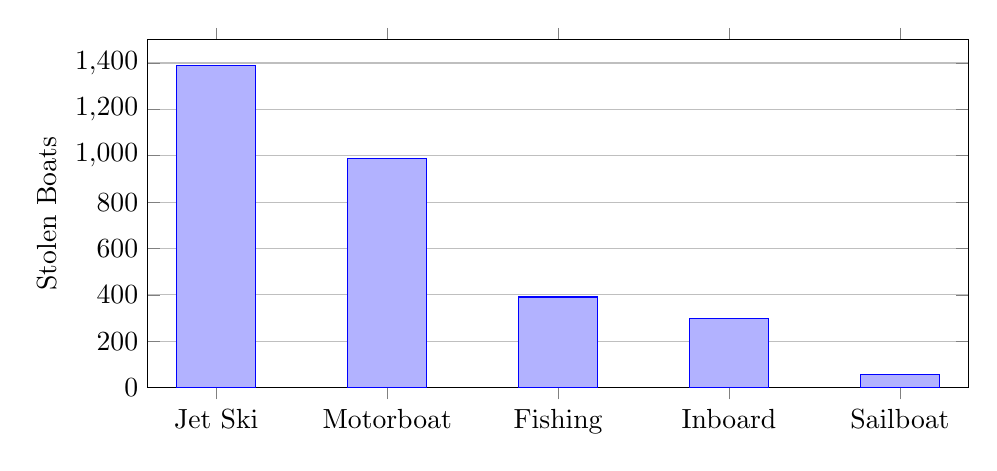
\begin{tikzpicture}
\begin{axis}[
%small,
height=6.0cm,
width=12.0cm,
%enlarge x limits=false,
%enlarge y limits=false,
%ybar interval,
ymajorgrids=true,
ylabel={Stolen Boats},
xlabel={},
bar width=1cm,
%x tick label style={rotate=0,anchor=center},
%xtick={120,140,...,1000},
%ytick={0,5,...,1000},
symbolic x coords={Jet Ski, Motorboat, Fishing, Inboard, Sailboat},
ybar,
ymin=0,
ymax=1500,
ytick={0,200,...,1500},
xtick=data,
%xmin=120,
%xmax=280,
%xticklabel style={/pgf/number format/.cd,fixed,precision=0},
%xticklabel=
%\pgfmathprintnumber\tick--\pgfmathprintnumber\nexttick
]
\addplot+
coordinates
{
(Jet Ski, 1389)
(Motorboat, 989)
(Fishing, 391)
(Inboard, 300)
(Sailboat, 56)
};
\end{axis}
\end{tikzpicture}
\end{center}\pause

Notice that for boat thefts, jet skis are the worst problem.
\end{example}
\end{frame}

\begin{frame}
\begin{definition}
A \textbf{frequency polygon} uses line segments connected to points located directly above class midpoint values.
\end{definition}\pause

\begin{definition}
A \textbf{relative frequency polygon} uses relative frequencies for the vertical scale.
\end{definition}\pause

\begin{block}{Features}
\begin{itemize}
\item Frequency polygons make it easy to compare two data sets.
\end{itemize}
\end{block}
\end{frame}

\definecolor{legend}{rgb}{0.9, 0.95, 0.9}
\begin{frame}
\begin{example}
The plot shows the wait times for both McDonald's and Dunkin' Donuts.
\begin{center}
\begin{tikzpicture}
\begin{axis}[
width=12cm,
height=6.3cm,
xlabel={Lunch Service Time (Seconds)},
ylabel={Frequency},
ytick={0,5,...,25},
xtick={24.5,49.5,99.5,...,349.5},
ymajorgrids=true,
xmajorgrids=true,
ymin=0,
ymax=25,
xmin=0,
xmax=360,
scatter/use mapped color={
 %draw=mapped color,
 %fill=blue,
},
legend style={fill=legend, fill opacity=1}
]
\addplot[scatter, blue, scatter src=y]
coordinates
{
(0.5, 0)
(49.5, 0)
(99.5, 11) 
(149.5, 23)
(199.5, 9)
(249.5, 3)
(299.5, 2)
(349.5, 0)
};
\addlegendentry{McDonald's}

\addplot[scatter, red, scatter src=y]
coordinates
{
(0.5, 0)
(49.5, 11)
(99.5, 22) 
(149.5, 14)
(199.5, 3)
(249.5, 0)
(299.5, 0)
(349.5, 0)
};
\addlegendentry{Dunkin' Donuts}
\end{axis}
\end{tikzpicture}
\end{center}
\end{example}
\end{frame}

\begin{frame}
\begin{block}{Pie Charts}
\vspace{4mm}
\begin{center}
\textbf{\LARGE
Never use pie charts.}
\end{center}

\vspace{0mm}
Not only are they a waste of ink, they lack an appropriate scale.
\end{block}\pause

\begin{block}{Note}
A Pareto chart will depict the same data, but better.
\end{block}
\end{frame}

\begin{frame}
\begin{block}{Nonzero Vertical Axis}
Always examine a graph carefully to see whether a vertical axis begins at some point other than zero so that differences are exaggerated.
\end{block}\pause

\begin{example}
\begin{center}
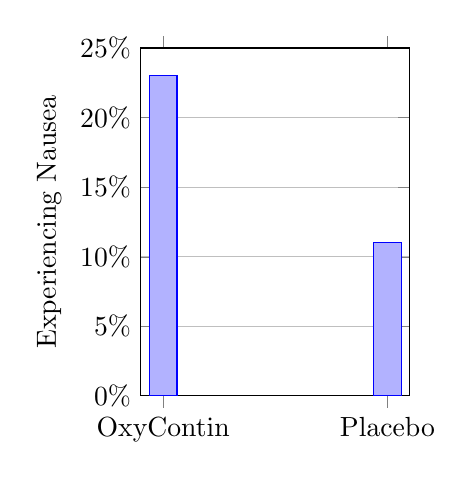
\begin{tikzpicture}
\begin{axis}[
%small,
height=6.0cm,
width=5.0cm,
%enlarge x limits=false,
%enlarge y limits=false,
%ybar interval,
ymajorgrids=true,
ylabel={Experiencing Nausea},
xlabel={},
%bar width=1cm,
%x tick label style={rotate=0,anchor=center},
%xtick={120,140,...,1000},
%ytick={0,5,...,1000},
symbolic x coords={OxyContin, Placebo},
ybar,
ymin=0,
ymax=25,
ytick={0,5,...,25},
xtick=data,
%xmin=120,
%xmax=280,
yticklabel style={/pgf/number format/.cd,fixed,precision=0},
yticklabel=
\pgfmathprintnumber\tick\%
]
\addplot+
coordinates
{
(OxyContin, 23)
(Placebo, 11)
};
\end{axis}
\end{tikzpicture}
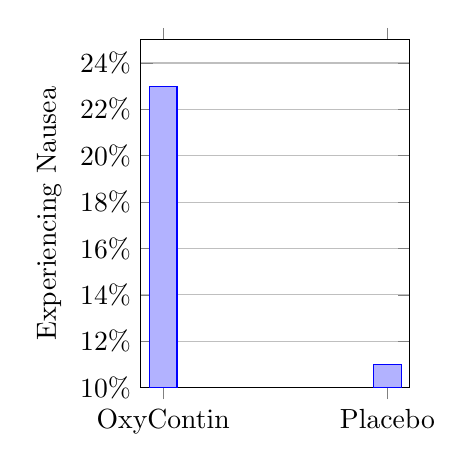
\begin{tikzpicture}
\begin{axis}[
%small,
height=6.0cm,
width=5.0cm,
%enlarge x limits=false,
%enlarge y limits=false,
%ybar interval,
ymajorgrids=true,
ylabel={Experiencing Nausea},
xlabel={},
%bar width=1cm,
%x tick label style={rotate=0,anchor=center},
%xtick={120,140,...,1000},
%ytick={0,5,...,1000},
symbolic x coords={OxyContin, Placebo},
ybar,
ymin=10,
ymax=25,
ytick={10,12,...,24},
xtick=data,
%xmin=120,
%xmax=280,
yticklabel style={/pgf/number format/.cd,fixed,precision=0},
yticklabel=
\pgfmathprintnumber\tick\%
]
\addplot+
coordinates
{
(OxyContin, 23)
(Placebo, 11)
};
\end{axis}
\end{tikzpicture}
\end{center}
\end{example}
\end{frame}

\begin{frame}
\begin{block}{Pictographs}
When examining data depicted with a pictograph, determine whether the graph is misleading because objects of area or volume are used to depict amounts that are actually one-dimensional.
\end{block}\pause

\begin{example}
The pictographs show data from the CDC\@.
\begin{figure}
\begin{subfigure}{.5\textwidth}
  \centering
  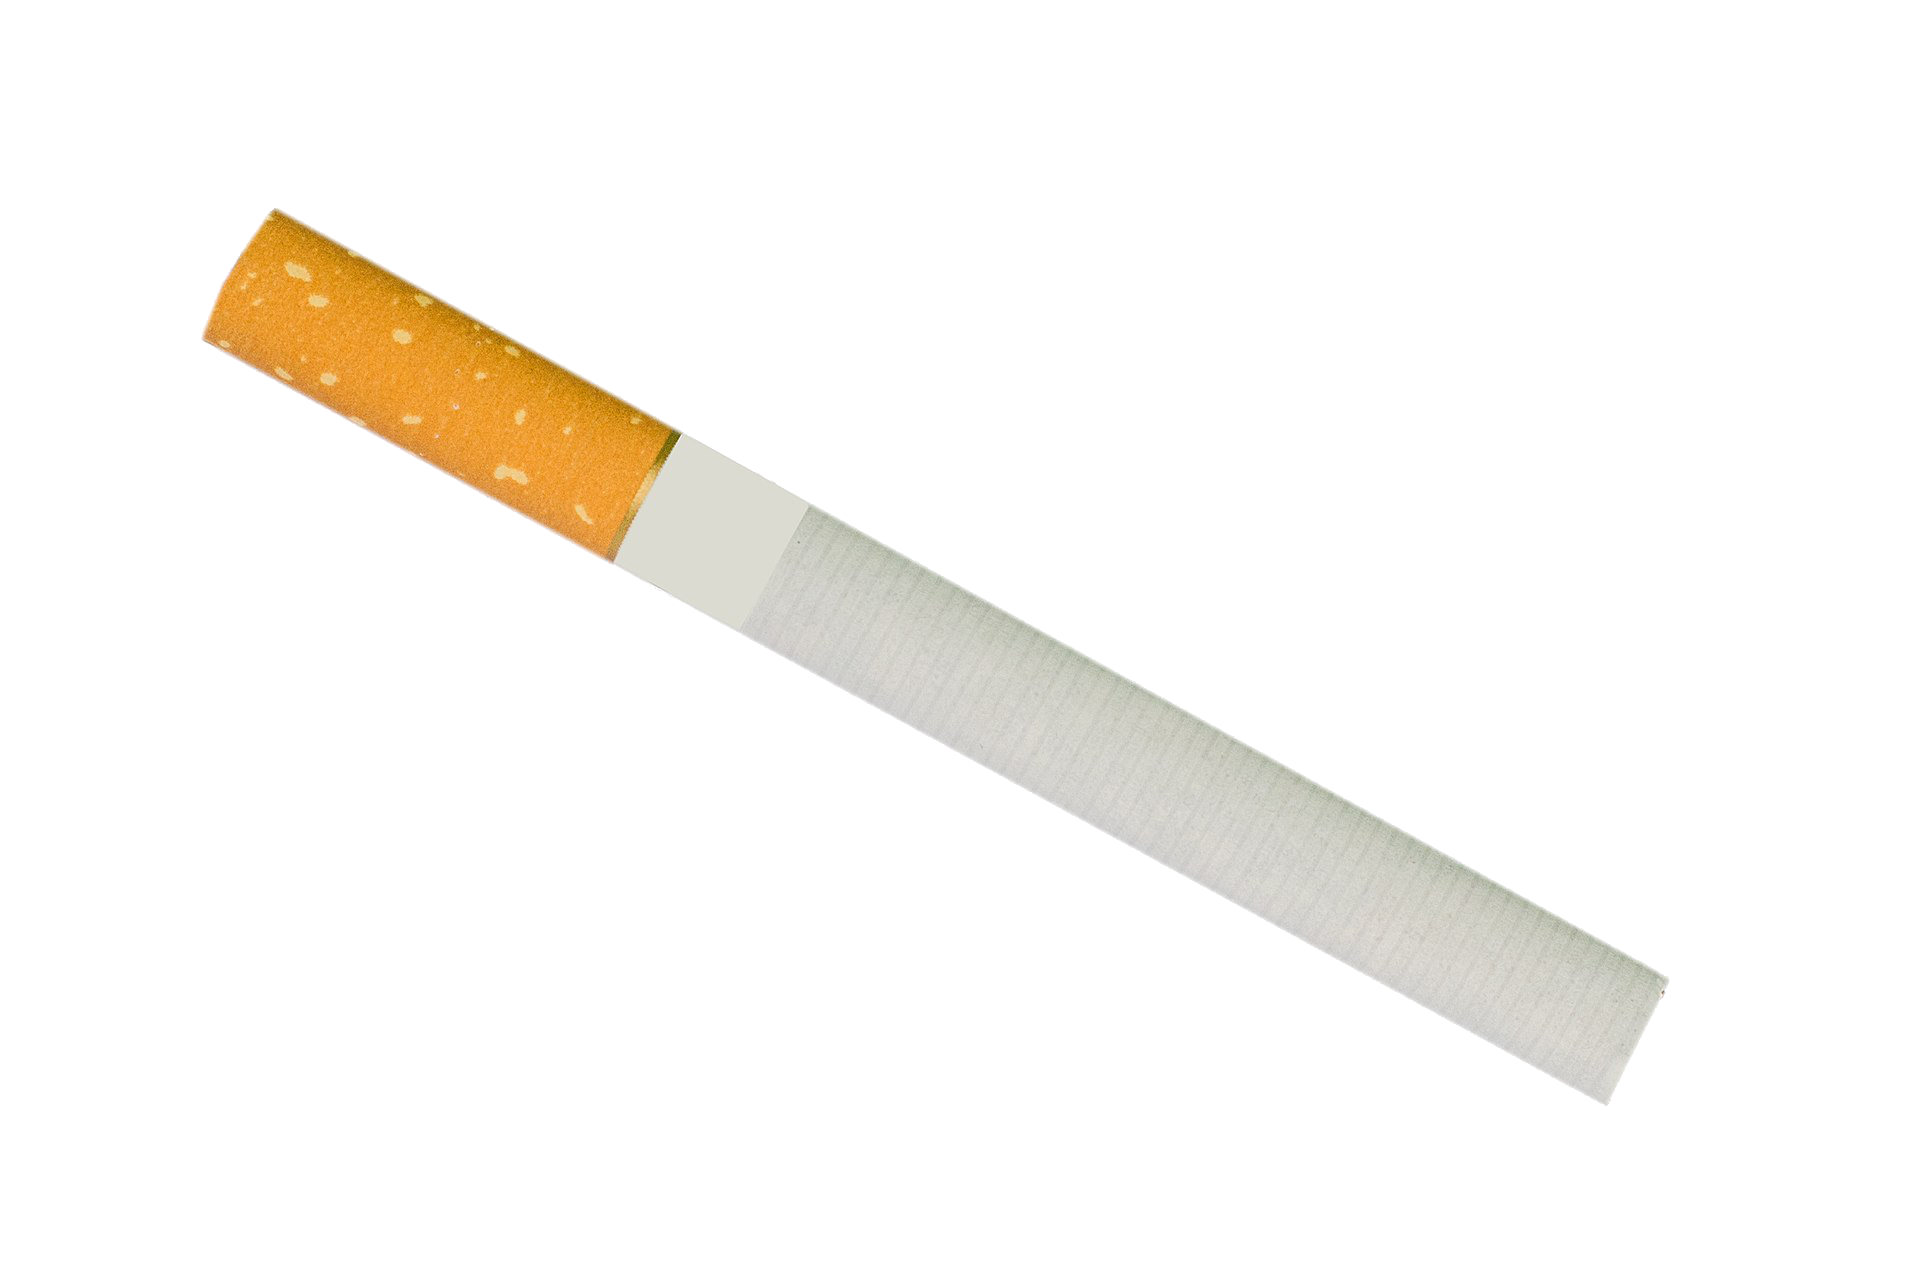
\includegraphics[width=.6\linewidth]{Cigarette.png}
  \caption{1970: 37\% of U.S. adults smoked.}
\end{subfigure}%
\begin{subfigure}{.5\textwidth}
  \centering
  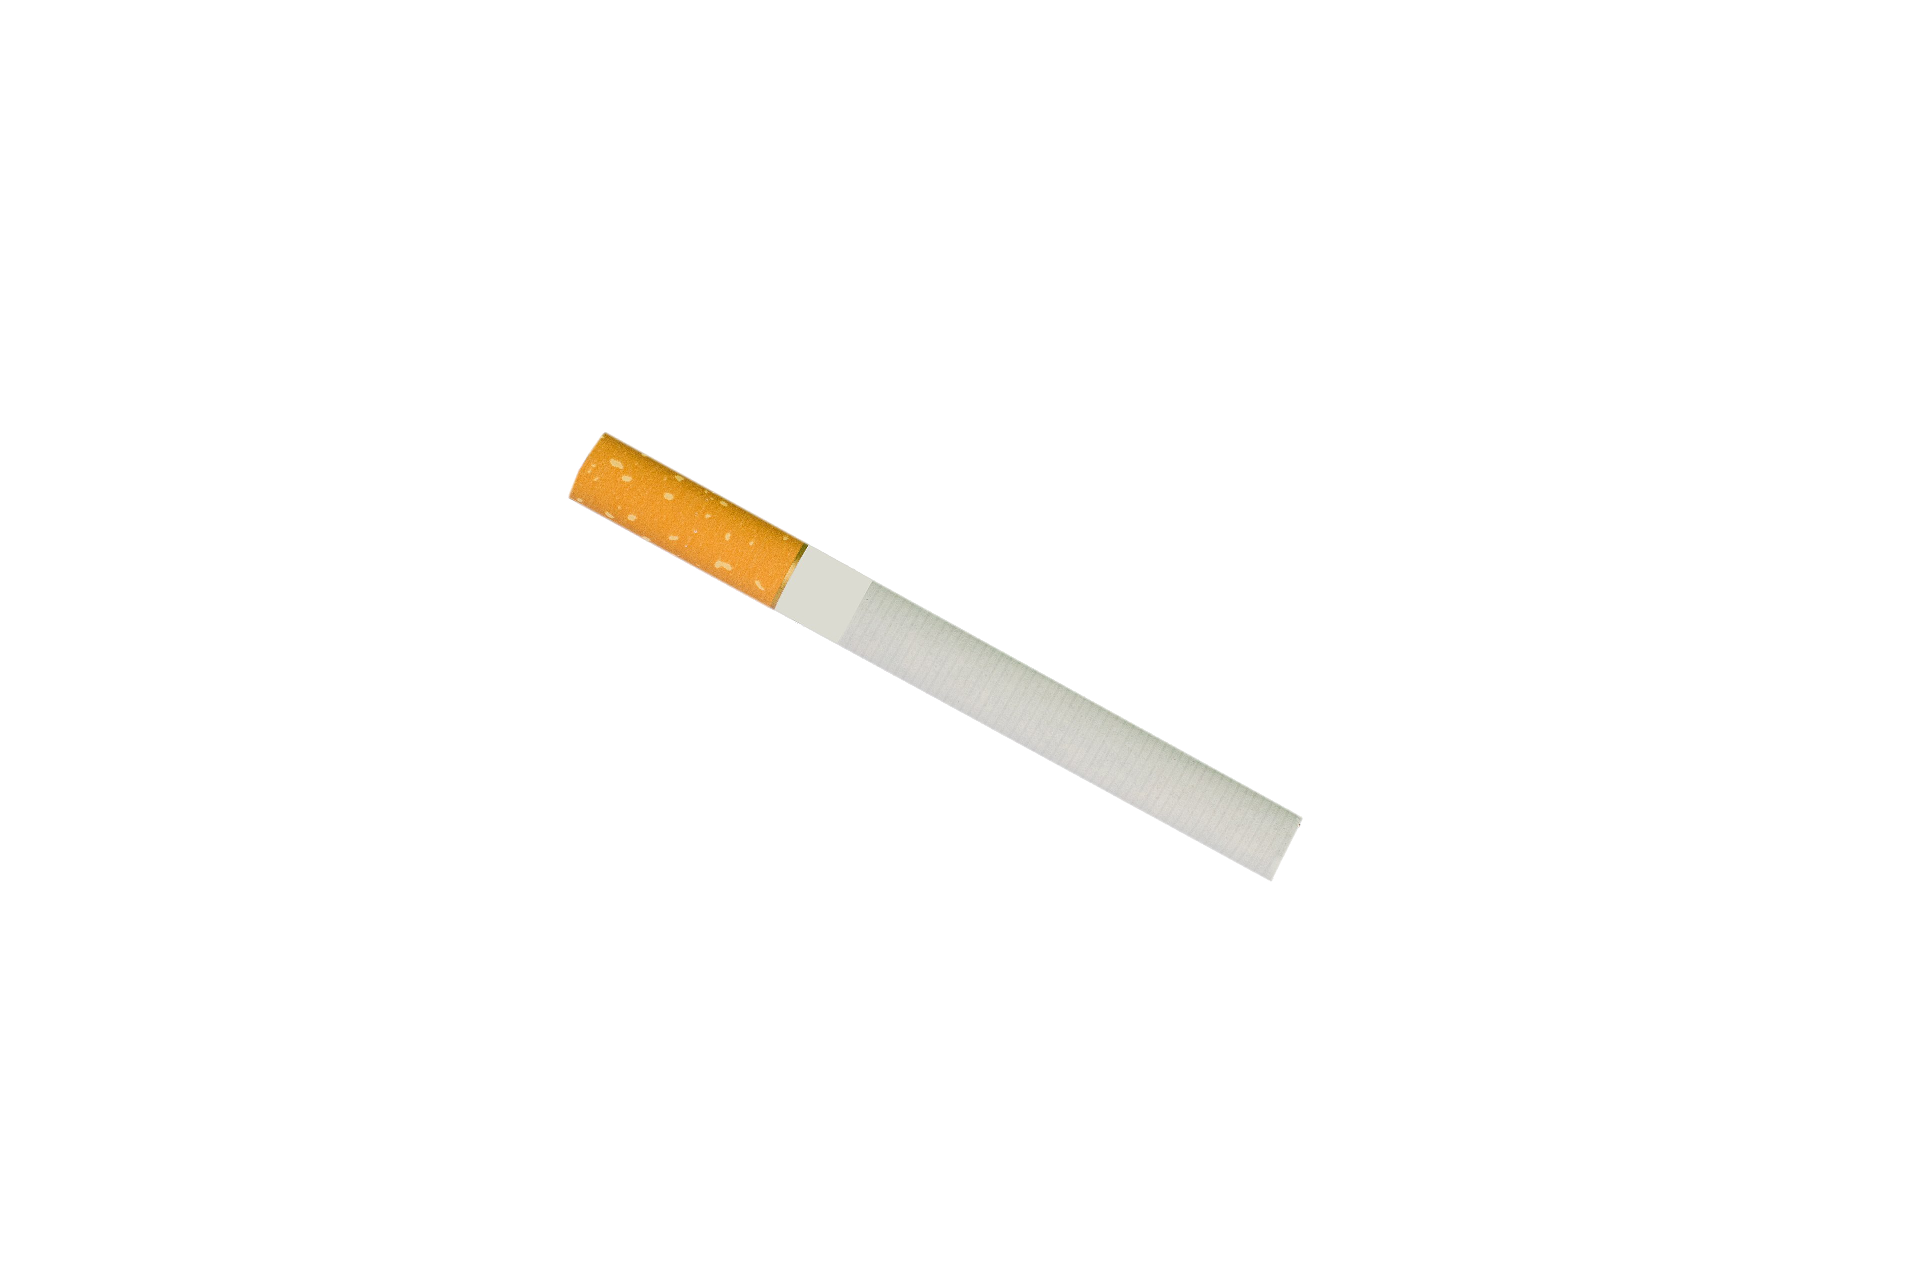
\includegraphics[width=.6\linewidth]{Cigarette_small.png}
  \caption{2013: 18\% of U.S. adults smoked.}
\end{subfigure}
\end{figure}
The larger cigarette is about twice as long as the smaller, which means it has four times the area of the smaller cigarette. While the data shows that 37\% is about twice of 18\%.
\end{example}
\end{frame}

\begin{frame}
\begin{block}{Final Notes}
\begin{itemize}[<+- | alert@+>]
\item For small data sets of 20 values or fewer, use a table instead of a graph.
\item A graph of data should make us focus on the true nature of the data, not on other elements, such as eye-catching but distracting design features.
\item Do not distort data. Construct a graph to reveal the true nature of the data.
\item Almost all of the ink in a graph should be used for data, not for other design elements.
\end{itemize}
\end{block}
\end{frame}
\end{document}
